\documentclass[
	english,
	fontsize=10pt,
	parskip=half,
	titlepage=true,
	DIV=12
]{scrartcl}

\usepackage[utf8]{inputenc}
\usepackage{babel}
\usepackage[T1]	{fontenc}
\usepackage{lmodern}
\usepackage{microtype}
\usepackage{color}
\usepackage{csquotes}

\usepackage{hyperref}

\usepackage{graphicx}
\usepackage{wrapfig}
\usepackage[bf]{caption}
	\captionsetup{format=plain}

\newcommand*{\tabcrlf}{\\ \hline}

\usepackage{amsmath}

\usepackage{minted}
	\usemintedstyle{friendly}

\newcommand*{\inPy}[1]{\mintinline{python3}{#1}}
\newcommand*{\ie}{i.\;e. }
\newcommand*{\eg}{e.\;g. }

\newcommand{\thus}{\ensuremath{\rightarrow}}

\begin{document}

\part*{Python Problems 09 (the last ones!), Spring 2021}

\section{Evaluating a Function (1 P)}
Create a NumPy-array that holds the values of $f(x)$ for 201 different $x \in [-3, +3]$. The values of $x$ should be equally spaced. For $f$, use:
\[ f(x) = \exp(-x^2) \cdot \sin(10x) \]
From this, create the following plot:
\begin{center}
	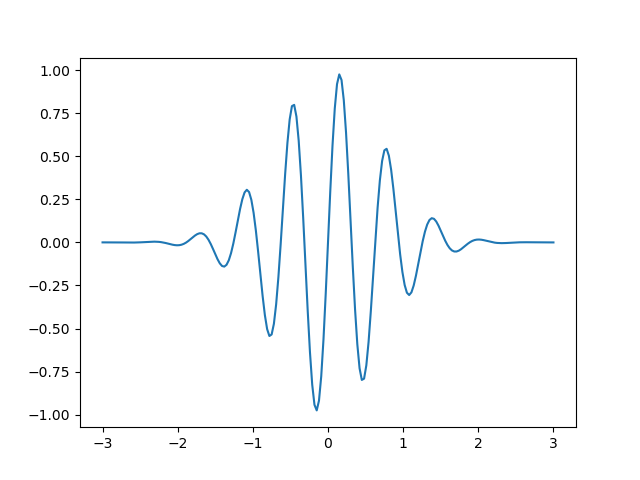
\includegraphics[width=.5\linewidth]{./task1}
\end{center}

\section{Block matrix (1 P)}
Create this matrix using NumPy-Functions:
\begin{minted}{text}
[[ 50  10   0   0   0   0   0   0   0   0   0   0   0   0   0   0   0   0]
 [ 10 100   0   0   0   0   0   0   0   0   0   0   0   0   0   0   0   0]
 [  0   0 150  20   0   0   0   0   0   0   0   0   0   0   0   0   0   0]
 [  0   0  20 200   0   0   0   0   0   0   0   0   0   0   0   0   0   0]
 [  0   0   0   0 250  30   0   0   0   0   0   0   0   0   0   0   0   0]
 [  0   0   0   0  30 300   0   0   0   0   0   0   0   0   0   0   0   0]
 [  0   0   0   0   0   0 350  40   0   0   0   0   0   0   0   0   0   0]
 [  0   0   0   0   0   0  40 400   0   0   0   0   0   0   0   0   0   0]
 [  0   0   0   0   0   0   0   0 450  50   0   0   0   0   0   0   0   0]
 [  0   0   0   0   0   0   0   0  50 500   0   0   0   0   0   0   0   0]
 [  0   0   0   0   0   0   0   0   0   0 550  60   0   0   0   0   0   0]
 [  0   0   0   0   0   0   0   0   0   0  60 600   0   0   0   0   0   0]
 [  0   0   0   0   0   0   0   0   0   0   0   0 650  70   0   0   0   0]
 [  0   0   0   0   0   0   0   0   0   0   0   0  70 700   0   0   0   0]
 [  0   0   0   0   0   0   0   0   0   0   0   0   0   0 750  80   0   0]
 [  0   0   0   0   0   0   0   0   0   0   0   0   0   0  80 800   0   0]
 [  0   0   0   0   0   0   0   0   0   0   0   0   0   0   0   0 850  90]
 [  0   0   0   0   0   0   0   0   0   0   0   0   0   0   0   0  90 900]]
\end{minted}

\emph{Hint}:\\
You can do so with only four lines of code. Look up \texttt{help(np.diag)}.

\emph{Background (Physics/Chemistry)}:\\
This is the Hamiltonian of a many-electron-system in the basis of their atomic orbitals. The eigenvalues of this matrix correspond with the energies of the binding and antibinding orbitals. While NumPy allows to find \emph{all} eigenvalues with a single comand, in practice you would extract the $^{N}/_{2}$ submatrices of dimension $2 \times 2$ along the principal diagonal. This is because matrix diagonalization takes $N^3$ steps. For big $N$ it is adavantageous to do $^{N}/_{2} \cdot 2^3 = 4N$ computations instead of $N^3$.

\section{Linear Optimization (3 P)}
You are craving sweets, but cannot spend more than 10\,€ on them. Your local dealer offers aldohexose\footnote{sugar! I swear, this simply means sugar!} containing compounds according to this price list:
\begin{itemize}
\item Dark chocolate -- 1.00\,€ per bar
\item Milk chocolate -- 0.90\,€ per bar
\item Caramel nuts bars -- 2.30\,€ per packet
\item Coco cubes -- 1.50\,€ per packet
\item Mint drops -- 0.30\,€ per bag
\end{itemize}

Taking package size and taste into account, you assign the following scores:
\begin{itemize}
\item Dark chocolate -- 5 points per bar
\item Mil, chocolate -- 4 points per bar
\item Caramel nuts bars -- 12 points per packet
\item Coco cubes -- 8 points per packet
\item Mint drops-- 1 point per bag
\end{itemize}

Write a program that tells you how to best convert  your money into $C_6H_{12}O_6$, \ie find out which configuration of sweets gives the highest score while still remaining within your budget.

\emph{Instruction}:\\
First, find out how much of each \emph{one} sweet you could buy. For each of these partial results $N_{\text{dark chocolate}}$, $N_{\text{milk chocolate}}, ...$ create a list like $L_{\text{milk chocolate}} = [0, 1, ..., N_{\text{milk chocolate}}]$. Use them to build a meshgrid.

\emph{Hint}:\\
You can build a meshgrid with an arbitrary number of dimensions. \texttt{X, Y, Z = np.meshgrid(ListX, ListY, ListZ)} works essentially the same way as in the 2D case shown in the lecture.

Using this meshgrid, you can now compute the total price and total score for each configuration. As you are well aware, many of the analyzed configurations are too expensive. Find those configurations surpassing the budget.

\emph{Hint}:\\
Using comparison operators, you can find all the too expensive configurations with a single line of code.

Overwrite the point score of the too expensive configurations such that they are rated as \inPy{-1}.

\emph{Hint}:\\
This, too, can be done in a single line of code.

Now use \texttt{np.argmax} with your score array. The result will be a single number, indicating the index in the \emph{flattened array}. Use the function  \texttt{np.unravel\_index} to reconstruct the indices of the multidimensional array. Look up the command here: \url{https://numpy.org/doc/stable/reference/generated/numpy.unravel_index.html}

\emph{Hint:}\\
The solution looks like this:
\begin{minted}{text}
Sugar-Strategy:
Sweet                | Count  | Price | Score 
---------------------+--------+-------+-------
dark chocolate       |      1 |  1.00 |   5.0
milk chocolate       |      0 |  0.00 |   0.0
caramel nuts bar     |      0 |  0.00 |   0.0
coco cubes           |      6 |  9.00 |  48.0
mint drops           |      0 |  0.00 |   0.0
---------------------+--------+-------+-------
TOTAL                |      7 | 10.00 |    53


Analyzed 157080 configurations.
\end{minted}

Congratulations! You have now solved a high-dimensional optimization problem! Sounds fancy, right?

\emph{Background}:\\
Problems of this kind are found frequently in real life. Here we used a \emph{brute force approach}, \ie we tried every single configuration. This will always work, but becomes impractical quickly. As you can see, for this little problem we already analyzed 157\,080 configurations; for any sweet included in our analysis, the effort increases roughly by a factor of 10\footnote{or better: by $\frac{\text{money}}{\text{average price of all sweets}}$}. We say, the problem has \emph{exponential time complexity in its number of components}.\\
\enquote{Better} approaches involve abstract maths which I cannot show you here. (In fact, I've taken the class \emph{Méthodes d'optimisation linéare} at the Université de Montpellier ... where I understood next to nothing). For small problems, however, you can easily adapt the solution you just found to solve new problems you might encounter. The power of Python is yours to use!
\end{document}
